\documentclass[]{standalone}
\usepackage{tikz}
\usepackage{pgffor}

\standaloneenv{tikzpicture}

\newcommand\colorWorldlayer{black}
\newcommand\colorLightcone{blue}
\newcommand\colorWorldline{red}
\newcommand\colorWorldlineII{green}

\newcommand\worldlineLength{5}
\newcommand\worldlineN{5}
\newcommand\worldlineDist{0.5}

\newcommand\drawWorldlines{
	\foreach \i in {0,...,\worldlineN}{	
		\draw[color=\colorWorldlayer] (0,\i*\worldlineDist) to (\worldlineLength,\i*\worldlineDist);
	}
}

\newcommand\drawWorldlayers{
	\foreach \i in {0,...,\worldlineN}{	
		\draw[color=\colorWorldlayer]
		(\worldlineDist,\i*\worldlineDist+\worldlineDist) to
		++(-\worldlineDist, -\worldlineDist) to
		++(\worldlineLength,0) to
		++(\worldlineDist, \worldlineDist);
	}
}

\newcommand\drawWorldlayersLabels{
	\foreach \i in {0,...,\worldlineN}{	
		\draw (-0.75, \i*\worldlineDist+0.2) node[anchor=east](){$t=\i$};
	}
}

\begin{document}
	
	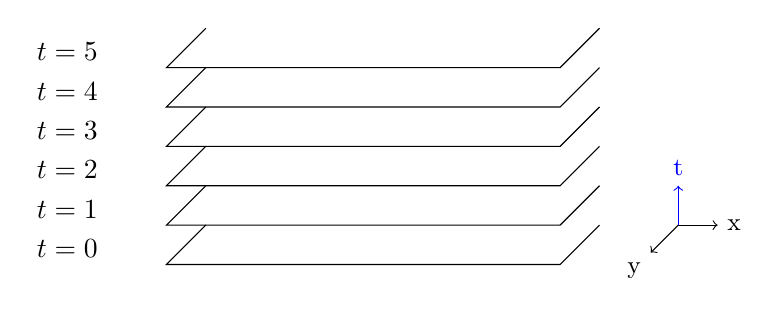
\begin{tikzpicture}
		
		\newcommand\coordinateSystemPosX{6.5}
		\newcommand\coordinateSystemPosY{0.5}
		\newcommand\coordinateSystemColX{black}
		\newcommand\coordinateSystemColY{black}
		\newcommand\coordinateSystemColT{blue}
		\newcommand\coordinateSystemArrowLen{0.5}
		
		\drawWorldlayers
		\drawWorldlayersLabels
	
		\draw[->, color=\coordinateSystemColX] (\coordinateSystemPosX, \coordinateSystemPosY) to ++(\coordinateSystemArrowLen, 0) node[anchor=west](){\small x};
		\draw[->, color=\coordinateSystemColY] (\coordinateSystemPosX, \coordinateSystemPosY) to ++(-\coordinateSystemArrowLen*0.7, -\coordinateSystemArrowLen*0.7) node[anchor=north east](){\small y};
		\draw[->, color=\coordinateSystemColT] (\coordinateSystemPosX, \coordinateSystemPosY) to ++(0, \coordinateSystemArrowLen) node[anchor=south](){\small t};
	\end{tikzpicture}
	
	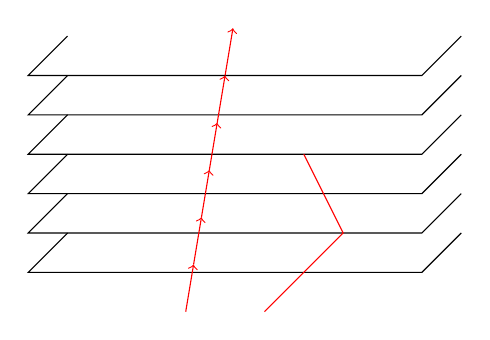
\begin{tikzpicture}
		\drawWorldlayers
		
		\newcommand\wlDX{0.1}
		\newcommand\wlDY{0.6}
		\foreach \i in {0,...,\worldlineN}{	
			\draw[->, color=\colorWorldline] (2+\wlDX*\i,-0.5+\wlDY*\i) to ++(\wlDX, \wlDY);
		}
	
		\draw[color=\colorWorldline]
			(3,-0.5) to[right, smooth] (4,0.5) to[smooth] (3.5,1.5);
	\end{tikzpicture}

	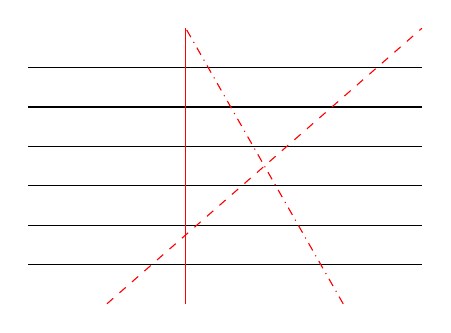
\begin{tikzpicture}
		\drawWorldlines
	
		\draw[color=\colorWorldline] (2,-0.5) to (2, 3);
		\draw[color=\colorWorldline, dashdotted] (4,-0.5) to (2, 3);
		\draw[color=\colorWorldline, dashed] (1,-0.5) to (5, 3);
	\end{tikzpicture}
	
	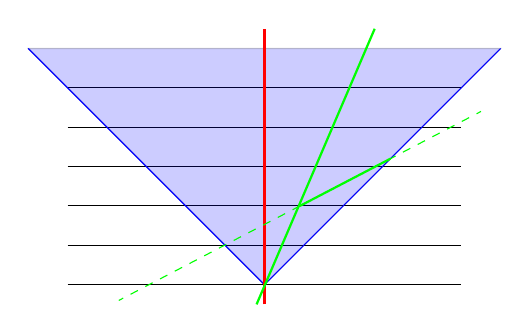
\begin{tikzpicture}
		\drawWorldlines
		
		\newcommand\lightconePosX{2.5}
		\newcommand\lightconePosY{0}
		\newcommand\lightconeHeight{3}
		\newcommand\lightconeHalfWidth{3}
		\newcommand\lightconeOpacity{0.2}
		
		\draw[fill=\colorLightcone, opacity=\lightconeOpacity]
			(\lightconePosX, \lightconePosY) to
			++(-\lightconeHalfWidth, \lightconeHeight) to
			++(+2*\lightconeHalfWidth, 0) to
			cycle;
		\draw[color=\colorLightcone]
			(\lightconePosX, \lightconePosY) to
			++(-\lightconeHalfWidth, \lightconeHeight);
		\draw[color=\colorLightcone]
			(\lightconePosX, \lightconePosY) to
			++(\lightconeHalfWidth, \lightconeHeight);
			
		\draw[color=\colorWorldline, thick] (\lightconePosX, \lightconePosY-0.25) to ++(0,3.5);
		\draw[color=\colorWorldlineII, thick] (\lightconePosX-0.1, \lightconePosY-0.25) to ++(1.5,3.5);

		\draw[color=\colorWorldlineII, thick] (2.95,1) to ++(1.15,0.6);
		\draw[color=\colorWorldlineII, dashed] (2.95,1) to ++(2.30,1.2);
		\draw[color=\colorWorldlineII, dashed] (2.95,1) to ++(-2.30,-1.2);
	\end{tikzpicture}

\end{document}